\pagebreak
\section{Sistema Input/Output}
Occupiamoci ora di un altro argomento molto importante. Stiamo parlando del sistema Input/Output che, nella maggior parte dei casi, è fondamentale per l'utilizzo dei computer. Spesso in fatto lo si utilizza non per la sua capacità computazionale ma per scrivere documenti, leggere dei \textit{files} da dispositivi, connettersi e navigare su internet oppure guardare un video. Tutte queste operazioni non hanno a che vedere con la potenza di calcolo del computer ma dalla capacità che ha quest'ultimo di integrare e connettere dispositivi esterni come periferiche di memorizzazione, schermi, tastiera, mouse, dispositivi per la connessione internet e molto altro. È proprio di questo che ci occuperemo in questo capitolo, di come il sistema operativo sia in grado di integrare questi dispositivi e riuscire a gestirli in maniera ottimale.

\subsection{Componenti hardware}
Passiamo ora all'analisi dei principali componenti HW. Come accennato in precedenza, possiamo spaziare da periferiche per la memorizzazione di dati, per la trasmissione oppure per la comunicazione con l'uomo (monitor, tastiera, mouse, etc).

Sono quindi presenti delle \textbf{porte}, ovvero i punti di connessione tra il dispositivo esterno e il computer. Internamente al calcolatore abbiamo dei \textbf{bus} che servono per la comunicazione tra la periferica e il computer o tra due periferiche. Tra i bus citiamo il bus \textbf{PCI}/PCIe, comunemente usati per la comunicazione tra schede e periferiche e sono ad elevate prestazioni (velocità e mole di dati). In secondo luogo abbiamo gli \textit{expansion bus} che servono per connettere periferiche più lente e le \textbf{SAS} (\textit{Serial Attached SCSI}) che sono comuni per i dischi. Osserviamo dalla figura \ref{fig:busses} che ci sono dei bus che sono direttamente collegati alla memoria tramite PCI mentre l'expansion bus è utilizzato per delle periferiche più lente.
\begin{figure}[h]
    \centering
    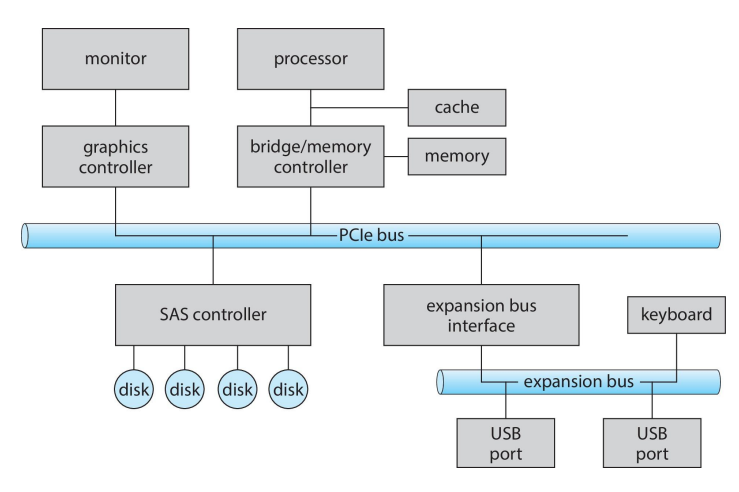
\includegraphics[width = .6\textwidth]{../res/imgs/IO system/busses.png}
    \caption{Illustrazione sui collegamenti tra periferiche.}
    \label{fig:busses}
\end{figure}

Sempre dall'immagine \ref{fig:busses} si osserva che i collegamenti sono generalmente gestiti da dei \textbf{controller}, che possono essere sia delle schede dedicate che integrate nel processore che interfacciano un componente con un altro.

% 
\subsection{Tecniche di comunicazione}
La comunicazione viene attraverso delle istruzione che sono scambiate con un set di registri che possono essere di quattro tipi:
\vspace{-5px}
\begin{itemize}
\setlength{\itemsep}{-.15 em}
    \item \textit{Data-in} e \textit{data-out} dove si possono rispettivamente ricevere e scrivere dati;
    \item \textit{Stato}, sono dei registri di stato che indicano se, per esempio, la comunicazione è stata effettuata correttamente o meno;
    \item \textit{Controllo} che servono effettivamente per inizializzare o modificare la comunicazione.
\end{itemize}
Questi registri, tipicamente vanno da 1 a 4 Byte. Spesso, al posto di fornire solamente un accesso al signolo registro, la periferica fornisce dei buffer Fifo dove viene incrementata la dimensione dei dati che è possibile leggere o scrivere. 

La trasmissione può essere effettuata mappando l'I/O del dispositivo nello spazio di indirizzamento del sistema operativo. In questo modo è possibile trasmettere comandi o dati sui registri andando a scrivere o leggere su indirizzi che sono uguali agli indirizzi di memoria. 
% 
\subsubsection{Polling}
Scaviamo più a fondo: come avviene la comunicazione input/output tra computer e una periferica? Il primo metodo che andiamo a vedere è quello dell'utilizzo di bit di diverso tipo:
\vspace{-5px}
\begin{itemize}
\setlength{\itemsep}{-.15 em}
    \item \textit{busy} bit, che indica se la periferica è libera o meno;
    \item \textit{read} o \textit{write} bit;
    \item \textit{command-ready} bit che controlla se ci sono dei comandi pronti ad essere eseguiti;
\end{itemize}
Segue un esempio di comunicazione con questa tecnica. Si controlla inizialmente se la periferica è occupata o meno attraverso il \textit{busy} bit. Nel caso la periferica è libera, imposta il modo di comunicazione attraverso il \textit{read/write} bit per poi impostare un comando e segnalare al controller che tale comando è pronto ad essere eseguito. A questo punto il controllore prenderà in considerazione il comando, imposta il \textit{busy} bit ad 1 e inizia l'esecuzione di tale comando.

Osserviamo che con il \textit{busy} bit si può verificare una situazione di \textit{busy-waiting}: il sistema operativo non può sempre controllare che una determinata periferica sia libera o meno. Se su 10000 volte, solo una volta il dispositivo è libero, si perde molto tempo per effettuare le 9999 richieste.

% 
\subsubsection{Interrupt}\label{interrupt handler}
Una soluzione sicuramente più ottimale comprende l'utilizzo di \textbf{interrupt}. In altre parole il sistema operativo effettua una richiesta ad una periferica, questa, appena sarà disponibile, la prenderà in considerazione e la completerà. Una volta completata, la periferica informa il sistema operativo attraverso un interrupt. Osserviamo che il sistema operativo non rimane fermo in attesa ma fa altre task per poi essere informato del soddisfacimento della richiesta. Una volta arrivato l'interrupt, questo è gestito dall'\textbf{interrupt handler} che è una \textit{routine}. Possiamo dividere gli interrupt in due categorie:
\vspace{-5px}
\begin{itemize}
\setlength{\itemsep}{-.15 em}
    \item Mascherabili (\textbf{maskable}) ovvero interrupt non critici e che possono essere messi in attesa;
    \item Non mascherabili (\textbf{nonmaskable}) che hanno una priorità maggiore (device non trovato) e che quindi devo essere serviti il prima possibili dalla CPU.
\end{itemize}

Gli interrupt non mascherabili, in quanto critici, sono divisi in molte sotto categorie, ognuna della quali deve essere gestita in maniera particolare. Ecco quindi che si è creata una tabella, l'\textbf{interrupt vector}, che per ogni tipo di interrupt assegna il numero dell'interrupt e l'interrupt \textit{handler} che lo andrà a gestire.
\begin{figure}[h]
    \centering
    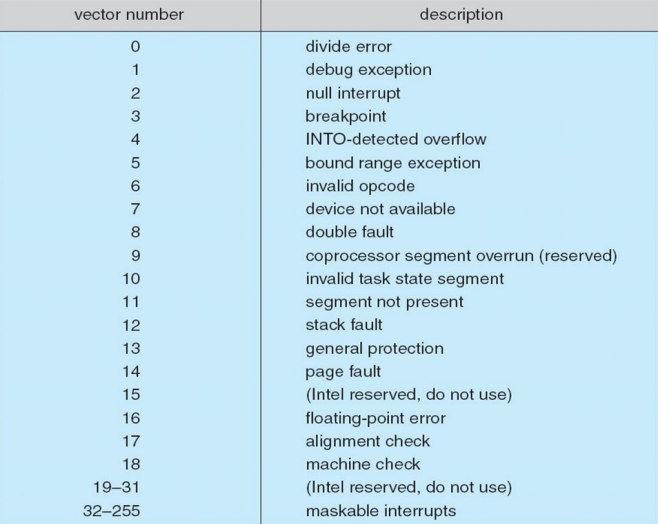
\includegraphics[width = .6\textwidth]{../res/imgs/IO system/interrupt_vector.png}
    \caption{Esempio della tabella di interrupt (Intel Pentium).}
    \label{fig:interruptVector}
\end{figure}
Dalla tabella in figura \ref{fig:interruptVector} osserviamo un esempio di interrupt vector: i primi 31 sono quelli non mascherabili e devono essere gestiti all'istante. Notiamo che tra i primi 31 è presente il \textit{page fault }(\ref{page fault}).

Si sottolinea, infine, che alcuni sistemi operativi come il \textit{Solaris}, sono in grado di gestire gli interrupt in maniera concorrente e parallela.

% 
\subsubsection{DMA}
Un uso intelligente dell'interrupt si ha nel DMA (\textit{Direct Memory Access}), che è quel controllore ormai integrato nei processori sessi che aiuta a gestire la comunicazione con \textit{devices} che richiedono un grosso flusso di scambio dati. Non siamo parlando di mouse e tastiera bensì di dischi rigidi o comunque in genere uno \textit{storage} secondario.

Come sappiamo, la CPU non usa i dati da qualsiasi periferica ma solo ed esclusivamente dalla memoria\footnote{Si intende, ovviamente, la memoria RAM.}. Di conseguenza un dato di un dispositivo esterno, al fine di essere utilizzato dal processore, deve innanzitutto passare dalla memoria. Conviene quindi lasciare questo compito al DMA che prende temporaneamente il controllo del bus tra CPU e memoria e gestisce la sincronizzazione con la periferica trasferendo i dati verso la periferica o verso la memoria (vedi figura \ref{fig:DMA}).
\begin{figure}
    \centering
    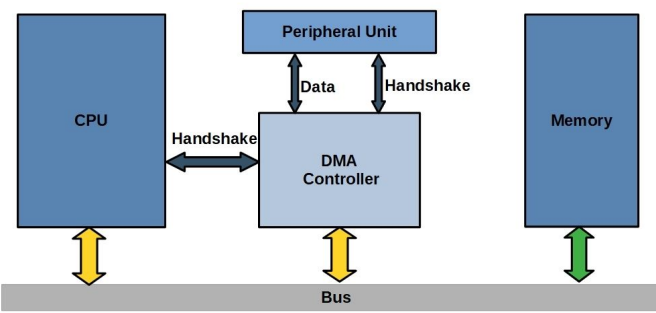
\includegraphics[width = .7\textwidth]{../res/imgs/IO system/DMA.png}
    \caption{Schema di funzionamento del DMA.}
    \label{fig:DMA}
\end{figure}
Nei sistemi di DMA più avanzati viene implementato anche lo scambio di dati tra periferica secondaria e memoria virtuale: si parla infatti di \textbf{DVMA}.

Più nel dettaglio, come fa il sistema operativo a sfruttare la potenza del DMA? Per prima cosa è necessario scrivere il comando su un blocco di memoria. In questo blocco di memoria, devono essere specificate le seguenti informazioni:
\vspace{-5px}
\begin{itemize}
\setlength{\itemsep}{-.15 em}
    \item \textit{Sorgente} (a quale periferica prelevare i dati) e la \textit{destinazione} dei dati (su quale blocco di memoria scriverli);
    \item Indicare se l'accesso è in lettura o scrittura;
    \item Dimensione di byte che devono essere letti, o scritti.
\end{itemize}
Dopo di che, all'interno del \textbf{DMA controller}, viene fornita la locazione in memoria del comando precedentemente scritto. A questo punto il DMA interpreta il comando fornito dal sistema operativo e gestisce il bus come richiesto. Il controllo del bus viene a tutti gli effetti rubato dalla CPU (\textit{cycle stealing}) ma viene creato un collegamento diretto - e veloce - tra periferica e memoria. Una volta terminato il trasferimento, il DMA, attraverso l'interrupt, segnala il tutto al sistema operativo.

% 
\subsection{Gestione software}\label{device-drivers}
Abbiamo discusso dell'hardware, abbiamo parlato della comunicazione tra il sistema operativo e le periferiche, ora saliamo di un livello e capiamo come l'input/output viene gestito a livello software dal \textit{kernel} del sistema operativo. Un approccio abbastanza diffuso è l'utilizzo di moduli dedicati a una o più periferiche: questi moduli sono detti \textbf{device-drivers}. Questi costituiscono un livello del \textit{kernel} che mette in comunicazione la parte software con la parte hardware del kernel. 

\subsubsection{Caratteristiche delle periferiche I/O} 
Nella gestione delle periferiche via software è importante tenere conto del tipo di periferica e del tipo di operazioni che tale periferica ci consente di fare. Inoltre è necessario tenere conto di alcune proprietà delle periferiche:
\vspace{-5px}
\begin{enumerate}
\setlength{\itemsep}{-.15 em}
    \item Se la comunicazione è a caratteri o a byte singoli;
    \item Se l'accesso di tipo sequenziale oppure \textit{random};
    \item Se si tratta di una comunicazione di tipo sincrono o asincrono (o eventualmente entrambi);
    \item Se si ha a che fare con periferiche condivise tra componenti oppure dedicate;
    \item Se la periferica è \textit{read-only}, \textit{write-only} oppure \textit{read-write};
    \item Se la velocità della periferica è ridotta (USB, bluetooth) oppure sostenuta (dal bus PCIe oppure le 100Gbit ethernet).
\end{enumerate}

% 
\subsubsection{Tipi di device-drivers}
I device-drivers devono quindi essere in grado di gestire la maggior parte dei meccanismo al fine di comunicare con il controllore della periferica. Possiamo dividere i device-drivers in quattro categorie, a seconda delle periferiche a cui si riferiscono: \textit{block devices} (dischi rigidi), \textit{character devices} (mouse e tastiera), \textit{memory-mapped I/O} (scheda grafica) e \textit{networking}.

\paragraph{Block devices} In questi \textit{drivers} la comunicazione avviene tramite bytes. I comandi tipici per interfacciarsi con i dispositivi ad essi associati (come i dischi rigidi) includono la lettura, la scrittura e la ricerca (\textit{seek}, ovvero il movimento della testina lungo i cilindri, vedi paragrafo \ref{seek}). Nel caso più comune si ha un \textit{file system} dedicato (capitolo \ref{file system}); altre volte invece si ha un accesso \textbf{raw}, ovvero lascia la possibilità all'applicazione stessa di accedere alla periferica in modo diretto (desiderabile da applicazioni che conoscono completamente l'architettura); infine si può avere un' accesso \textbf{diretto} dove il sistema operativo garantisce dei privilegi all'applicazione ma mantiene comunque un controllo per quel \textit{device} per qualche altro processo. È molto comune l'uso di \textit{memory-mapped file}, ovvero associare dei file in aree del disco in modo tale che accedere ad un file equivale ad accedere ad una locazione in memoria. Questi drivers, dato che si interfacciano con il disco, sono quelli che fanno maggiormente uso del \textbf{DMA}.

\paragraph{Character devices} Questi driver sono invece associati a tastere o mouse che sono più lente e quindi richiedono uno scambio di dati meno consistente. Spesso la comunicazione in lettura e scrittura avviene attraverso dei comandi dedicati come \texttt{get} oppure \texttt{put}.

\paragraph{Networking} Visto l'importanza di tali drivers, questi hanno una classe a parte. L'interfaccia software con cui si comunica con tali periferiche viene chiamata \textbf{socket}: interfaccia il sistema operativo a tali \textit{devices}. Oltre alla comunicazione networking tra \textit{devices}, il socket può essere utilizzato per \textit{inter-process comuncation}, la comunicazione tra processi diversi all'interno della stessa macchina.

\paragraph{Clock e timer} Sono molto utili per mantenere la data del sistema oppure per generare degli interrupt periodici (utilizzati nel Round Robin, paragrafo \ref{RR}). Attraverso dei protocolli dedicati, come l'\textit{NTP}, sincronizzare diversi computer su una rete per fare in modo che questi siano allinaeati tutti con la stessa data, correggendo eventuali sfasamenti.

% 
\subsubsection{Device sincroni e asincroni}
Un'importante caratteristica dei \textit{devices} che abbiamo elencato è se questi siano sincroni o asincroni, in particolare, per quanto riguarda i sincroni, se questi sono \textbf{blocking} e \textbf{non}blocking.

\paragraph{Blocking} una comunicazione di questo tipi si ha quando, dopo una richiesta di lettura o scrittura su una periferica ed, effettivamente blocchiamo l'esecuzione del codice su quell'istruzione, fino a che la richiesta non è soddisfatta. Questo tipo di comunicazione è ottima se ad ogni richiesta è quasi garantita una risposta; altrimenti si ricade nel \textit{busy-waiting}.

\paragraph{Nonblocking} In questo caso il device non fornisce tutti i dati che sono stati richiesti ma fornisce i dati che sono disponibili al momento della richiesta (alcuni magari stanno per essere sovrascritti da un altro processo). Immaginiamo un \textit{device} con un \textit{buffer} e ogni volta che riceve una richiesta, fornisce solo il contenuto del buffer.

\paragraph{Asincrono} Nella modalità asincrona, la gestione del \textit{device}, al posto di effettuare continui check, si utilizzano gli interrupt. In questo caso il processore continua a lavorare fino a che non riceve l'interrupt. 

% 
\subsection{Task del kernel}
Nella gestione dell'I/O il kernel deve essere in grado di fornire funzione per accodare e soddisfare richieste di processi diversi associati a periferiche diverse che possono essere condivise o meno. Ovviamente, quando si ha a che fare con situazioni come questa, dove sono presenti code di processi, si avranno sicuramente degli algoritmi di \textbf{scheduling} al fine di ottimizzare le tempistiche e soddisfare in modo equo le richieste dei processi verso le periferiche. Ad esempio, nel caso della comunicazione asincrona, il kernel si affida alla \textbf{device-status table} (figura \ref{fig:device-status table}) che è una tabella che contiene lo stato delle periferiche.
\begin{figure}[h]
    \centering
    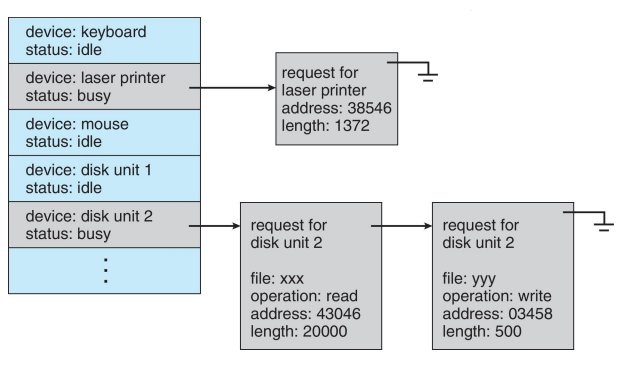
\includegraphics[width = .65\textwidth]{../res/imgs/IO system/device-status table.png}
    \caption{Device-status table che, per ogni periferica, ha collegata la coda contenente i processi in attesa.}
    \label{fig:device-status table}
\end{figure}
Per ogni periferica, e quindi per ogni riga della tabella, il kernel collega la coda dei processi che sono in attesa del \textit{device}.

Ricordiamo che tutte le comunicazioni tra periferiche e il computer avvengono tramite il sistema operativo: di conseguenza il kernel deve anche implementare dei metodi di \textit{buffering} in modo da equilibrare la velocità della periferica con la velocità di CPU. A volte si usano anche dei metodi più sofisticati come il \textit{double buffering} che ritorna utile nel caso di periferiche con diversa velocità: in un buffer processa i dati con velocità ridotta rispetto al secondo in modo da non rallentare la velocità della periferica. 

\subsubsection{Gestione degli errori}
naturalmente il sistema operativo deve essere in grado di gestire anche gli \textbf{errori} e di uso errato da parte delle periferiche. Tipicamente quando andiamo a fare delle chiamate per accedere ad una periferica, avremo a che fare con dei messaggi di errore: se vale 0, l'accesso è andato a buon fine, altrimenti il numero identifica l'errore che si è verificato. Il sistema operativo deve essere in grado di gestire questi errori, possibilmente tenendone traccia attraverso dei \textbf{file di log}. 

Tutta la gestione dell'I/O è fatta in maniera \textbf{priviegiata} dal kernel per cui se l'utente vuole accedere ad una periferica, per farlo dobbiamo utilizzare delle \textit{system calls} che fanno la richieste al kernel che a sua VOLA richiede al device. In particolare la \textit{system call} genera un interrupt che viene catturato dal sistema operativo, viene interpretato, prende i dati richiesti dall'utente e li restituisce. C'è sempre un passaggio dal kernel per accedere ad una periferica. 

% 
\subsubsection{Strutture dati}
Ovviamente il kernel fornisce anche delle strutture dati. Le strutture più significative sono tabelle per la gestione di file aperti, connessioni di rete e anche verificare lo stato di alcuni devices. Sono incluse anche strutture dati che tengono traccia di buffers, allocazioni di memoria o se determinati blocchi sono stati sovrascritti o meno (\textit{dirty blocks}).

Si osserva che su sistemi operativi Linux e Unix è possibile accedere alle periferiche in maniera concettualmente simile all'accesso del file. Su Windows, invece, la gestione della comunicazione I/O è effettuata principalmente mediante dei \textbf{messaggi} che concettualmente sono più semplici, ma sono fonte di \textit{overhead} oerchè sono più complessi da gestire

\subsubsection*{Gestione dell'energia}
La gestione dell'energia non è un argomento inerente - e per questo non approfondito - alla gestione dell'I/O ma rimane legato. Ci limitiamo ad ossorvare che nei sistemi moderni ci sono dei meccanismo come le \textbf{ACPI} (\textit{Advanced Configuration and Power Interface}) che è un \textbf{firmware} che fornisce \textit{routines} utilizzate dal kernel per gestire al meglio non solo l'energia del dispositivo ma anche la gestione di nuove periferiche e la gestione degli errori.

Sappiamo che la gestione dell'energia è un \textit{key factor} per i dispositivi mobile. In questi dispositivi il sistema operativo fornisce dei meccanismi aggiuntivi per la il \textit{power management} in modo anche da utilizzare in maniera ottimizzata le risorse. Tra questi meccanismo si citano i \textbf{wake-loks}, di Android, che servono per fare in modo che il sistema operativo non vada in \textit{sleep mode}. Si pensi ad un video che stiamo guardando sul nostro telefono; generalmente il telefono, se inutilizzato, si blocca dopo alcuni minuti: in questo caso però, dato che si sta guardando un video i \textit{wake locks} fanno in modo che il sistema operativo non vada in \textit{sleep-mode} mentre si sta guardando il video. Una volta terminato, i wake locks vengono rilasciati.

\subsubsection*{Performance}
Per gestire tutte le periferiche, il sistema operativo, assieme all'hardware, deve effettuare un numero elevato di operazioni, anche solo per fare una banale operazione di lettura o scrittura. Ecco quindi che ha senso tenere conto di tutti questi meccanismo nel momento in cui si va a progettare un \textit{device-driver}. Delle buone pratiche per aumentare le performance sono:
\vspace{-5px}
\begin{itemize}
\setlength{\itemsep}{-.15 em}
    \item Ridurre il numero di \textit{context-switches}: ogni volta che un processo si mette in attesa genera un context switch dove parte un altro processo che a sua volta può mettersi in wait etc;
    \item Ridurre la copia di dati: i processi devo sempre richiedere i dati tramite il kernel, significa che tali dati devono prima essere copiati nel kernel e poi passati all'utente;
    \item Ridurre il numero di interrupt;
    \item Cercare di usare il più possibile funzionalità come il DMA;
\end{itemize}

Generalmente, nella progettazione si parte dall'implementazione di alcuni algoritmi livello applicativo. Una volta testati possono essere passati al kernel in modo da renderli più efficiente fino a poi essere parte integrante del controller dove si va proprio a modificare il firmware stessi. Al caso ottimale si arriva alla soluzione hardware dove cresce l'efficienza ma decresce, ovviamente, il livello di flessibilità.
